\chapter{Introduction} \label{ch:introduction}

\section{Concept and Motivation}
% What are we trying to get done here?
Humanoid robots are great, and we want to get things done with them.
We ended up doing navigation and crawling.
% Navigating a humanoid robot.
Navigating a humanoid is necessary if we want to get the robot to do things
that aren't where it already is.
Get there to manipulate, create a map of environment, survey, etc.
% Crawling a humanoid robot.
Crawling can give the robot access to places where it can't walk.
Crawling is more stable.
Crawling can get you under things.
Crawling can get you over difficult terrain.
% Why are we trying to get these things done?
% Navigating is a fundamental thing for mobile robots.
% Crawling gives the robot another mode of locomotion and allows it to get to
% more places.

\begin{figure}[h!]
	\centering
    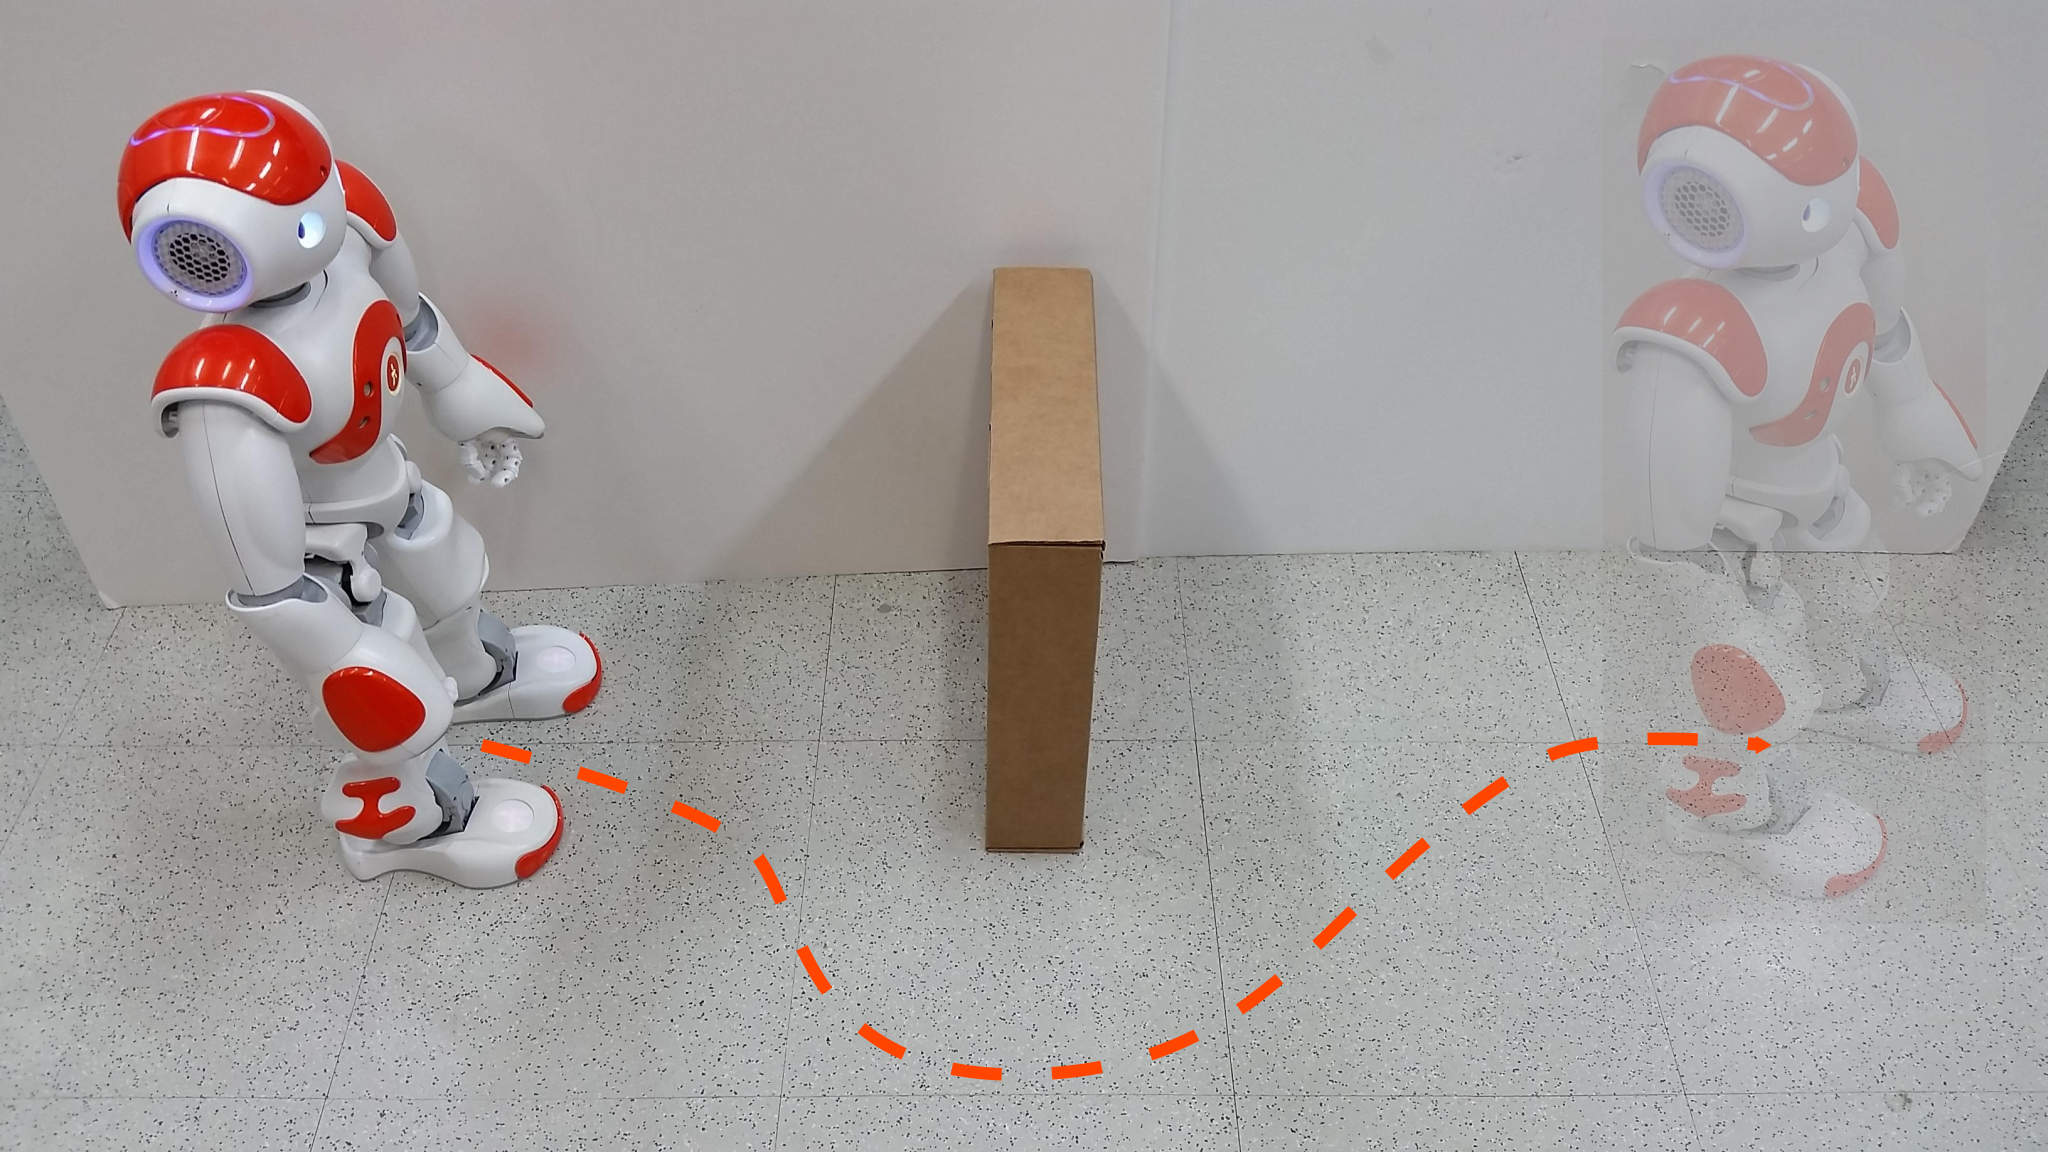
\includegraphics[width=0.7\textwidth]{nao_with_obstacle2.pdf}
	\caption{Example illustration of the Nao humanoid robot in an environment 
             with an obstacle. The red X represents a goal location with the 
             blue arrows showing an possible path. On the left side is one 
             possible representation of the environment as a 2D grid.}
	\label{fig:nao_with_obstacle2}
\end{figure}

\section{Background}
% Review previous work here as well.
% Why humanoids?
Humanoid platforms are very adaptable. Various terrains. 
Humanoids can locomote and manipulate.
Humanoids are compatible with our humanoid orient environment.
People relate to humanoids.
% Who's done humanoids before?
When was the first humanoid?
 - WABOT-1 1970
 Ichiro Kato, “Development of biped walking robot WABOT-1,” Biomechanism 2, pp.173-214,
 1973 (in Japanese).
Notable humanoids:
- QRIO https://www.techfak.uni-bielefeld.de/~rhaschke/lehre/WS04/humanoids/papers/qrio-mechanics.pdf
- DARWIN http://www.romela.org/wp-content/uploads/2015/05/Development-of-open-humanoid-platform-DARwIn-OP.pdf
- Nao http://lars.mec.ua.pt/public/LAR%20Projects/Humanoid/2011_RicardoGodinho/Pesquisa%20Disserta%C3%A7%C3%A3o/Mechatronic%20design%20of%20NAO%20humanoid.pdf
- iCub http://vislab.isr.ist.utl.pt/publications/07-JAR-icub-compress.pdf

Big boys
- ASIMO
- ATLAS
- Robonaut
- Valkyrie.

 Stuff that has been done with humanoids:
Walking gaits
 - zero moment point
DRC, HRI with the Nao.
% What is the problem of navigating, briefly.
Navigation is fundamental. Get the robot somewhere safely. Otherwise it might
as well not be mobile.
Layered approach.
% Who's done navigation?
Search based planners: ASTAR, RRT, other search.
Continuous planners: Potential field, Backstepping, DWA, Feedback Linearization
% We've done navigation.
Our Nao paper on GODZILA\@.
Original GODZILA paper.
% What is the problem of crawling, briefly.
Call it, humanoid quadrupedal locomotion.
More stable than walking, can deal with more terrains, can get you under things.
% Who's done crawling?
CPG actor critic paper. Maybe there's another one?
% We've done crawling.
Our paper on crawling.

\section{Platform Overview}

\begin{figure}
	\centering
	\includegraphics[width=0.4\textwidth]{nao_coronal_highlighted2.png}
    \caption{Coronal view of the Nao humanoid with a few pertinent features 
             highlighted.}
	\label{fig:nao_diagram1}
\end{figure}

% What equipment did we use?
% - Nao
% - Lidar
% - Mount
We used a Nao. What's that?
We used a Lidar. What's that? We used a Hokuyo. What's that?
We made a mount.

% Why did we use these things?
We used a Nao, because it's a humanoid.
We used a Lidar because you can see more things.
We had to make a mount to get it on there.


\section{GODZILA Navigation}
% Briefly, what's navigation?
% What approach did we go for?
% Why did we go for this?
GODZILA is a potential field local approach.
Potential field is this blah.
It's cheap on memory and fast to compute.
It's local. Now we can build more on top of it.

\section{Projected Profile Crawl Gait}
% Briefly, what's crawling?
% Why crawling?
% What approach did we go for?
% Why did we go for this approach?
Statically stable.
You take the robot as symmetric and do a saggital projection.
Can compose the gait into two modes.
Applicable to other platforms.

\section{Thesis Structure}
This thesis is organized as follows: 

% Chapter \ref{ch:platform} reviews the Nao Humanoid Platform with Hokoyu Scanning Laser Rangefinder augmentation.
% The navigation system is broken into three parts, 
% Chapter \ref{ch:navigation} discusses the GODZILA algorithm used for local navigation.
% Chapter \ref{ch:crawl_gait} discusses the Projected Profile crawling gait used to perform the crawl.
% Simulations and experimental results are shown in Chapters \ref{ch:simulations} and \ref{ch:results}, 
% while a discussion of the work is given in Chapter \ref{ch:conclusion}.
